\documentclass{beamer}
%
% Choose how your presentation looks.
%
% For more themes, color themes and font themes, see:
% http://deic.uab.es/~iblanes/beamer_gallery/index_by_theme.html
%
\mode<presentation>
{
  \usetheme{default}      % or try Darmstadt, Madrid, Warsaw, ...
  \usecolortheme{default} % or try albatross, beaver, crane, ...
  \usefonttheme{default}  % or try serif, structurebold, ...
  \setbeamertemplate{navigation symbols}{}
  \setbeamertemplate{caption}[numbered]
} 

\usepackage[english]{babel}
\usepackage[utf8x]{inputenc}
\usepackage[font=small]{caption}
\graphicspath{ {./img/} }

\title[PR1/2 Demo]{PR1/2 Demo}
\author{Christian Permann}
\institute{Faculty of Computer Science, University of Vienna,\newline W\"ahringer Stra{\ss}e 29, 1090 Vienna}
\date{11.12.2018}

\begin{document}

\begin{frame}
  \titlepage
\end{frame}

% Uncomment these lines for an automatically generated outline.
%\begin{frame}{Outline}
%  \tableofcontents
%\end{frame}

\section{Introduction}

\begin{frame}{Milestones}

\begin{itemize}
  \item Basic tool with visualization of existing data. (PR1) (done)
  \item Enable running (ELKI) algorithms from the custom tool. (done)
  \item Properly save and display clustered data. (done, missing saving of results)
  \item Enable defining presets and running multiple clusterings. (done)
  \item Allow for parameter space exploration within results. (OPTICS)

\end{itemize}

\end{frame}

\section{Tool}

\begin{frame}{The Tool}

\centerline{Demo}

\end{frame}

\section{New Interfaces}

\begin{frame}{More Interfaces}

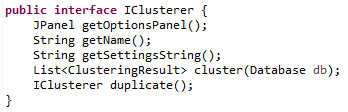
\includegraphics[width=0.53\textwidth]{interface1}
\captionof{figure}{The interface for clustering algorithms}
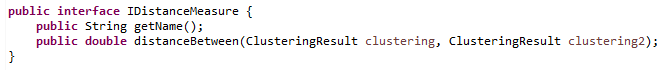
\includegraphics[width=\textwidth]{interface2}
\captionof{figure}{The interface for meta distance-measures}

\end{frame}

\section{Introduction}

\begin{frame}{What we have}

The good:
\begin{itemize}
  \item OPTICS seems to work well, clusters represented in MDS plot.
  \item The chosen distance measures give quite similar looking results $\rightarrow$ validate each other.
\end{itemize}
The bad:
\begin{itemize}
  \item Nothing can be saved yet. ELKI classes not serializeable - object references when rebuilding from custom format?
\end{itemize}
The ugly:
\begin{itemize}
  \item The colors are the same between selected clustering and meta-clustering.
  \item The colors are sometimes ugly when there are lots of clusters. 
\end{itemize}

\end{frame}

%\bibliography{citations}
\bibliographystyle{ieeetr}

\end{document}